%==============================================================
%  Figura 8.4 - Diagramma a blocchi (Esempio 1)
%  Adattamento in italiano della Figura 8.4 dell'IFA Report 2/2017
%
%  Coordinate ricavate dal disegno di partenza (1 cm = 70 px,
%  origine all'estremita' sinistra della linea di collegamento).
%==============================================================
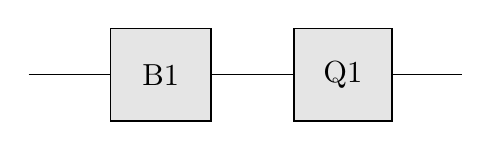
\begin{tikzpicture}[
  font=\normalsize,
  filo/.style={draw=black, line width=0.6pt},
  blocco/.style={draw=black, line width=0.6pt, fill=black!10},
  etichetta/.style={inner sep=1pt, scale=1.1}
]

% Linea di collegamento
\draw[filo] (0,0) -- (1.043,0);
\draw[filo] (2.314,0) -- (3.371,0);
\draw[filo] (4.614,0) -- (5.500,0);

% Blocchi
\draw[blocco] (1.043,-0.586) rectangle (2.314,0.586);
\draw[blocco] (3.371,-0.586) rectangle (4.614,0.586);

\node[etichetta] at (1.679,0) {B1};
\node[etichetta] at (3.993,0) {Q1};

\end{tikzpicture}
